% Basic drawings
% https://www.sharelatex.com/blog/2013/08/27/tikz-series-pt1.html
% https://www.tug.org/TUGboat/tb29-1/tb91walczak.pdf
\documentclass[border=3pt,tikz]{standalone}

\usepackage{tikz}
\begin{document}

\begin{tikzpicture}
  \draw (0,0) -- (4,0) -- (4,4) -- (0,4) -- (0,0);
\end{tikzpicture}



\begin{tikzpicture}
  \draw[red,thick,dashed] (2,2) circle (3cm);
\end{tikzpicture}



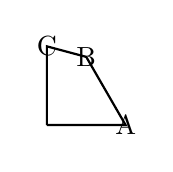
\begin{tikzpicture}

\draw[thick] (0,0)
%    polar coordinate     name  text
  -- (0:1) node at (0:1) (R1-0) {A}
  -- (60:1) node at (60:1) (R1-60) {B}
  -- (90:1) node at (90:1) (R1-90) {C}
  -- (0,0);

\end{tikzpicture}



\begin{tikzpicture}

\draw[->] (0:0.5)
   arc[start angle=-90, end angle=180, radius=1cm] node[left] {$\psi$};
   
\end{tikzpicture}




\begin{tikzpicture}

\draw[->]
  (0:0.5) arc (-90:180:1) node[left] {$\psi$};
   
\end{tikzpicture}



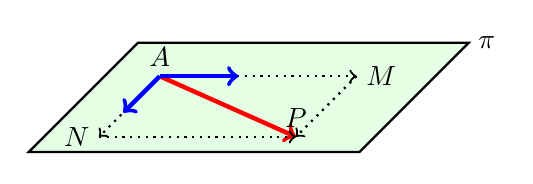
\begin{tikzpicture}
  % Note: the points have coordinates (x,z,y)
  \coordinate (O) at (0,0,0);
  \coordinate (P0) at (3,2,2);
  \coordinate (P) at (5.5,2,4);

  % Points M i N
  \coordinate (M) at (5.5,2,2);
  \coordinate (N) at (3,2,4);

  % Points of directing vectors

  \coordinate (V1) at (4,2,2);
  \coordinate (V2) at (3,2,3.2);

  % Points of the plane from A, P, M and N
  \coordinate (PLA0) at (2.3,2,0.9);
  \coordinate (PLA1) at (6.5,2,0.9);
  \coordinate (PLA2) at (2.3,2,4.5);
  \coordinate (PLA3) at (6.5,2,4.5);      

  % Plane
  \fill[color=green!10,thick,draw=black] (PLA0) -- (PLA1) -- (PLA3) -- (PLA2) -- cycle;
  \draw (PLA1) node[anchor=west] {$\pi$};

  % Points: A, P and position vector and AP
  \draw[color=red,ultra thick,->] (P0) -- (P);
  \draw (P0) node[anchor=south] {$A$};
  \draw (P) node[anchor=south] {$P$};

  % Parallelogram law
  \draw[thick, dotted,->] (P0) -- (M);
  \draw[thick, dotted,->] (P0) -- (N);
  \draw[thick, dotted,->] (M) -- (P);
  \draw[thick, dotted,->] (N) -- (P);         

  % Points M and N and their vectors
  \draw[ultra thick,color=blue,->] (P0) -- (V1);
  \draw[ultra thick,color=blue,->] (P0) -- (V2);
  \draw (M) node[anchor=west] {$M$};
  \draw (N) node[anchor=east] {$N$};
\end{tikzpicture}



\end{document}